% Preamble
	\documentclass[12pt,a4paper]{article} % Article type document
% Packages
	\usepackage[utf8]{inputenc} % utf8
	\usepackage{amsmath} % Math
	\usepackage[T1]{fontenc} % Fonts
	\usepackage{amsfonts} % Math
	\usepackage{amssymb} % Math
	\usepackage[spanish,es-tabla]{babel} % Languages
	\usepackage{makeidx} % Makeidx
	\usepackage{hyperref} % Links
	\usepackage{graphicx} % Graphs
	%\usepackage{subfig} % Using in conjunction with subcaption creates a conflict
	\usepackage{cite} % Cite
	\usepackage{natbib} % Bibliography
	\usepackage{lmodern} % Lmodern
	\usepackage{listings} % Listings
	\usepackage{xcolor} % Colours
	\usepackage{float} % Figure
	\usepackage{xfrac} % Frac
	\usepackage{fix-cm} %
	\usepackage{setspace} % Setspace
	\usepackage{fancyhdr} % Fancy
	\usepackage{lipsum} % Text
	\usepackage{appendix} % Appendix
	\usepackage{tikz} % Figure
	\usepackage{caption} % Caption
	\usepackage{subcaption} % Using in conjunction with subfig creates a conflict
	\usepackage{titlesec} % To customize titles, sections, etc.
	\usepackage{booktabs} % Table
	\usepackage{pgf-pie} % Pie graphs
% Document customization
	\captionsetup[table]{
		name = Tabla,
		labelsep = newline,
		justification = raggedright,
		singlelinecheck = false,
		labelfont = bf
	}
	\renewcommand{\thesection}{\Roman{section}}
	\renewcommand{\thesubsection}{\arabic{section}.\arabic{subsection}}
	\AtBeginDocument{\renewcommand{\contentsname}{\textcolor{red!85}{ÍNDICE}}}
	\onehalfspace
	\fancyhead[L]{}
	\fancyhead[C]{}
	\fancyhead[R]{}
	\fancyfoot[L]{}
	\fancyfoot[C]{}
	\fancyfoot[R]{\thepage}
	\renewcommand{\headrulewidth}{0pt}
	\renewcommand{\footrulewidth}{0pt}
	\graphicspath{{Imagenes/}}
	\usepackage[margin = 2.54cm]{geometry} % Geometry
	\setlength{\parindent}{0cm} % Sangría
	% Define colors
		\definecolor{gris}{gray}{0.9}
		\definecolor{azul}{rgb}{0.0, 0.48, 0.65}
	% Customize sections
		\titleformat{\section}
			{\bfseries\large}
			{\large\thesection.\hspace{0.5mm}}
			{1pt}
			{}
		\titlespacing{\section}
			{0pt}
			{3.5ex plus 1ex minus .2ex}
			{2.3ex plus .2ex}
	% Customize for programs code	
		\definecolor{codegreen}{rgb}{0,0.6,0}
		\definecolor{codegray}{rgb}{0.5,0.5,0.5}
		\definecolor{codepurple}{rgb}{0.58,0,0.82}
		\definecolor{backcolour}{rgb}{0.95,0.95,0.92}
		\lstdefinestyle{mystyle}{
			backgroundcolor=\color{backcolour},   
			commentstyle=\color{codegreen},
			keywordstyle=\color{magenta},
			numberstyle=\tiny\color{codegray},
			stringstyle=\color{codepurple},
			identifierstyle=\color{blue},
			basicstyle=\ttfamily\footnotesize,
			breakatwhitespace=false,         
			breaklines=true,                 
			captionpos=b,                    
			keepspaces=true,
			numbers=left,                    
			numbersep=5pt,                  
			showspaces=false,                
			showstringspaces=false,
			showtabs=false,                  
			tabsize=2
		}
		\lstset{style=mystyle}
	% Customize with hypersetup
		\definecolor{linkcolorred}{HTML}{FF3333}
		\definecolor{urlcolorblue}{HTML}{336BFF}
		\hypersetup{pdfstartview=FitH, 
					linkcolor= linkcolorred, 
					urlcolor=urlcolorblue,
					citecolor = blue, 
					colorlinks=True} 	
% Document
\begin{document}
	\pagestyle{empty}
	% Carátula
	\begin{titlepage}
		\begin{center}
			{\textbf{UNIVERSIDAD}}\\
			{\textbf{FACULTAD}}\\
			{\textbf{ESCUELA PROFESIONAL}}\\
			\vspace{2cm}
			\begin{figure}[h]
				\centering
				
\includegraphics[height=7cm]{logo-unsch.png}
			\end{figure}
			\vspace{2mm}
			\begin{center}
				{\textbf{TÍTULO DE LA TESIS}}
			\end{center}
			\vspace{1cm}
				{\bf Tesis}\\
			\vspace{2mm}
				{\textit{Bachiller o título profesional}}\\
			\vspace{1cm}
				{\bf Autor}\\
			\vspace{2mm}
				{Nombre completo del autor}\\
			\vspace{4mm}
				{\bf Asesor}\\
			\vspace{2mm}
				{Nombre completo del asesor}\\
			\vspace{16mm}
				{CIUDAD, AÑO}\\
			\vspace{2mm}
				{PAÍS}
		\end{center}
	\end{titlepage}
	\newpage % Nueva página
		\setcounter{page}{1}
		\pagestyle{fancy} % Estilo de página
		\tableofcontents % Tabla de contenidos
		\textcolor{red!85}{\listoffigures}  % Índice de figuras
		\textcolor{red!85}{\listoftables} % Índice de tablas
	\newpage % Nueva página
	% Introducción
	\section*{INTRODUCCIÓN}
	\addcontentsline{toc}{section}{INTRODUCCIÓN}
		\lipsum[1-3]
		Según \cite{Schmidt-2020}, describe
		\lipsum[4]
	% Planteamiento del problema
	\newpage
	\section{PLANTEAMIENTO DEL PROBLEMA}
		%% Enunciado del problema
		\subsection{Enunciado del problema}
			\lipsum[4]
			Como mensiona \cite{Koop-2003}, en su libro
			\lipsum[5]
		%% Formulación del problema
		\subsection{Formulación del problema}
			\lipsum[5]
			%%% Problema general
			\subsubsection{Problema general}
				\lipsum[6]
			%%% Problemas específicos
			\subsubsection{Problemas específicos}
				\lipsum[1]
				Un texto es una composición de signos codificados en un sistema
				de escritura que forma una unidad de sentido. También es una composición
				de caracteres imprimibles generados por un algoritmo de cifrado que, aunque no
				tienen sentido para cualquier persona, sí puede ser descifrado por su destinatario original.
				\begin{enumerate}
					\item Un texto es una composición de signos codificados en un sistema
					de escritura que forma una unidad de sentido.
					\item Un texto es una composición de signos codificados en un sistema
					de escritura que forma una unidad de sentido.
					\item Un texto es una composición de signos codificados en un sistema
					de escritura que forma una unidad de sentido.
					\item Un texto es una composición de signos codificados en un sistema
					de escritura que forma una unidad de sentido.
				\end{enumerate}
	% Objetivos
	\newpage
	\section{OBJETIVOS}
		%% Objetivo general
		\subsection{Objetivo general}
			\lipsum[8]
		%% Objetivos específicos
		\subsection{Objetivos específicos}
			\lipsum[9]
			\lipsum[10]
			\lipsum[11]
	% Justificación
	\newpage
	\section{JUSTIFICACIÓN}
		\lipsum[10]
		\lipsum[11]
		\lipsum[12]
		\lipsum[13]
		\lipsum[14], es por ello la relevancia
		de este trabajo de investigación \citep{Takayama-1985}
	% Marco teórico
	\newpage
	\section{MARCO TEÓRICO}
	Como se menciona en el trabajo de \cite{Johnson-1987}, la revisión de \lipsum[10]
	Consider the following first-order vector difference equation: 
		\begin{equation}\label{eq: MED}
			\left[
				\begin{array}{c}
					y_{t}  \\
					y_{t-1}\\
					y_{t-2}\\
					\vdots \\
					y_{t-p+1}
				\end{array}
			\right] =
			\left[
				\begin{array}{cccccc}
					\phi_{1} & \phi_{2} & \phi_{3} & \cdots & \phi_{p-1} & \phi_{p}\\
					    1    &    0     &    0     & \cdots &      0     &     0   \\
					    0    &    1     &    0     & \cdots &      0     &     0   \\
					 \vdots  &  \vdots  &  \vdots  & \cdots &   \vdots   &  \vdots \\
					    0    &    0     &    0     & \cdots &      1     &     0   \\
				\end{array}
			\right]
			\left[
				\begin{array}{c}
					y_{t-1}\\
					y_{t-2}\\
					y_{t-3}\\
					\vdots \\
					y_{t-p}
				\end{array}
			\right] + 
			\left[
				\begin{array}{c}
					w_{t}\\
					0    \\
					0    \\
				  \vdots \\
				    0
				\end{array}
			\right]
		\end{equation}
		%% Marco histórico
		\subsection{Marco histórico}
			\lipsum[11].
			\begin{equation}\label{eq: LAG1}
				y_{t} = (a + bL)Lx_{t}
			\end{equation}
			is exactly the same as
			\begin{equation}\label{LAG2}
				y_{t} = (aL + bL^{2})x_{t} = ax_{t-1} + bx_{t-2}
			\end{equation}
			To take another example, 
			\begin{equation}\label{eq: LAG3}
				\begin{aligned}
					(1-\lambda_{1}L)(1-\lambda_{2}L)x_{t} &= 
					(1-\lambda_{1}L-\lambda_{2}L + \lambda_{1}\lambda_{2}L^{2})x_{t}\\
					                                      &= 
				    (1-\left[\lambda_{1}+\lambda_{2}\right]L + \lambda_{1}\lambda_{2}L^{2})x_{t}\\
					                                      &= 
				    x_{t}-(\lambda_{1} + \lambda_{2})x_{t-1} + (\lambda_{1}\lambda_{2})x_{t-2}
				\end{aligned}
			\end{equation}
		%% Sistema teórico
		\subsection{Sistema teórico}
			\lipsum[12].
			Gráfica estadisticas:
			\begin{figure}[H]
				\centering
				\begin{tikzpicture}[scale = 1.2]
					\pie{10/{NSP}, 20/{Aprobados}, 30/{Retirados}, 35/{Jalados}, 5/{Susti con fe}}
				\end{tikzpicture}
				\caption{Resultados}
				\label{fig: Pie}
			\end{figure}
		%% Marco conceptual
		\subsection{Marco conceptual}
			\lipsum[13]
		%% Marco referencial
		\subsection{Marco referencial}
			\lipsum[14]
	% Hipótesis
	\newpage
	\section{HIPÓTESIS}
	Las hipótesis son una respuesta tentativa 
	como señala \cite{Das-2019} \lipsum[14]
		%% Hipótesis general
		\subsection{Hipótesis general}
			\lipsum[15]		
		%% Hipótesis específicos
		\subsection{Hipótesis específicos}
			\begin{enumerate}
				\item Un texto es una composición de signos codificados en un sistema
				de escritura que forma una unidad de sentido.
				\item Un texto es una composición de signos codificados en un sistema
				de escritura que forma una unidad de sentido.
				\item Un texto es una composición de signos codificados en un sistema
				de escritura que forma una unidad de sentido.
				\item Un texto es una composición de signos codificados en un sistema
				de escritura que forma una unidad de sentido.
			\end{enumerate}
	% Variables e indicadores
	\newpage
	\section{VARIABLES E INDICADORES}
	\lipsum[17], es relevante el análisis de las variables e indicadores como señala \cite{Carter-1958}
		% Tabla
		\begin{table}[ht]
			\raggedright
			\caption{Variables e indicadores}
			\begin{tabular}{cc}
				\toprule
				Variables & Indicadores \\
				\midrule
				Variable 1 & Indicador 1\\
				Variable 2 & Indicador 2\\
				Variable 3 & Indicador 3\\
				Variable 4 & Indicador 4\\
				\bottomrule
			\end{tabular}
			\vspace{2mm}
			\caption*{\it Nota: Elaboración propia.}
			\label{tab: Variables e indicadores 1}
		\end{table}
		\lipsum[1]
		\begin{table}[ht]
			\raggedright
			\caption{Variables e indicadores}
				\begin{tabular}{cc}
					\toprule
					Variables & Indicadores \\
					\midrule
					Variable 1 & Indicador 1\\
					Variable 2 & Indicador 2\\
					Variable 3 & Indicador 3\\
					Variable 4 & Indicador 4\\
					\bottomrule
			\end{tabular}
			\vspace{2mm}
			\caption*{\it Nota: Elaboración propia.}
			\label{tab: Variables e indicadores 2}
		\end{table}	
	% Metodología
	\newpage
	\section{METODOLOGÍA}
		\lipsum[1-4]. 
		\newpage
		The population mean $\mu$ is also called the \textit{expectation}
		of $X$, denoted $E(X)$ or sometimes simply $EX$. In general,
		the expectation of a function $g(X)$ is given by
			\begin{equation}
				E\left(g\left(X\right)\right) =
				\int\limits_{-\infty}^{\infty}g(x)f_{x}(x)dx,
			\end{equation}
		where $f_{x}(x)$ is the density of $X$. For example, the $r$th population moment of $X$ is the expectation of $X^{r}$.
		
		Consider the random variable $ a + bX$ for constants $a$ and $b$.
		Its expectation is 
			\begin{equation}
				\begin{aligned}
					E\left(a+bX\right) &= \int_{-\infty}^{\infty}
					\left[a + bx\right]\cdot f_{x}(x)dx \\
					&= a\int_{-\infty}^{\infty}f_{x}(x)dx  + 
					b\int_{-\infty}^{\infty}x\cdot f_{x}(x)dx\\
					&= a + bE(X)
				\end{aligned}
			\end{equation}
		\lipsum[1]
		\begin{equation}\label{eq: MLG}
			Y_{i} = \beta_{1} + \beta_{2}X_{2i} + \cdots + \beta_{k}X_{ki} + \mu_{i}
		\end{equation}
		\lipsum[1]
		\begin{figure}[h]
			\centering
			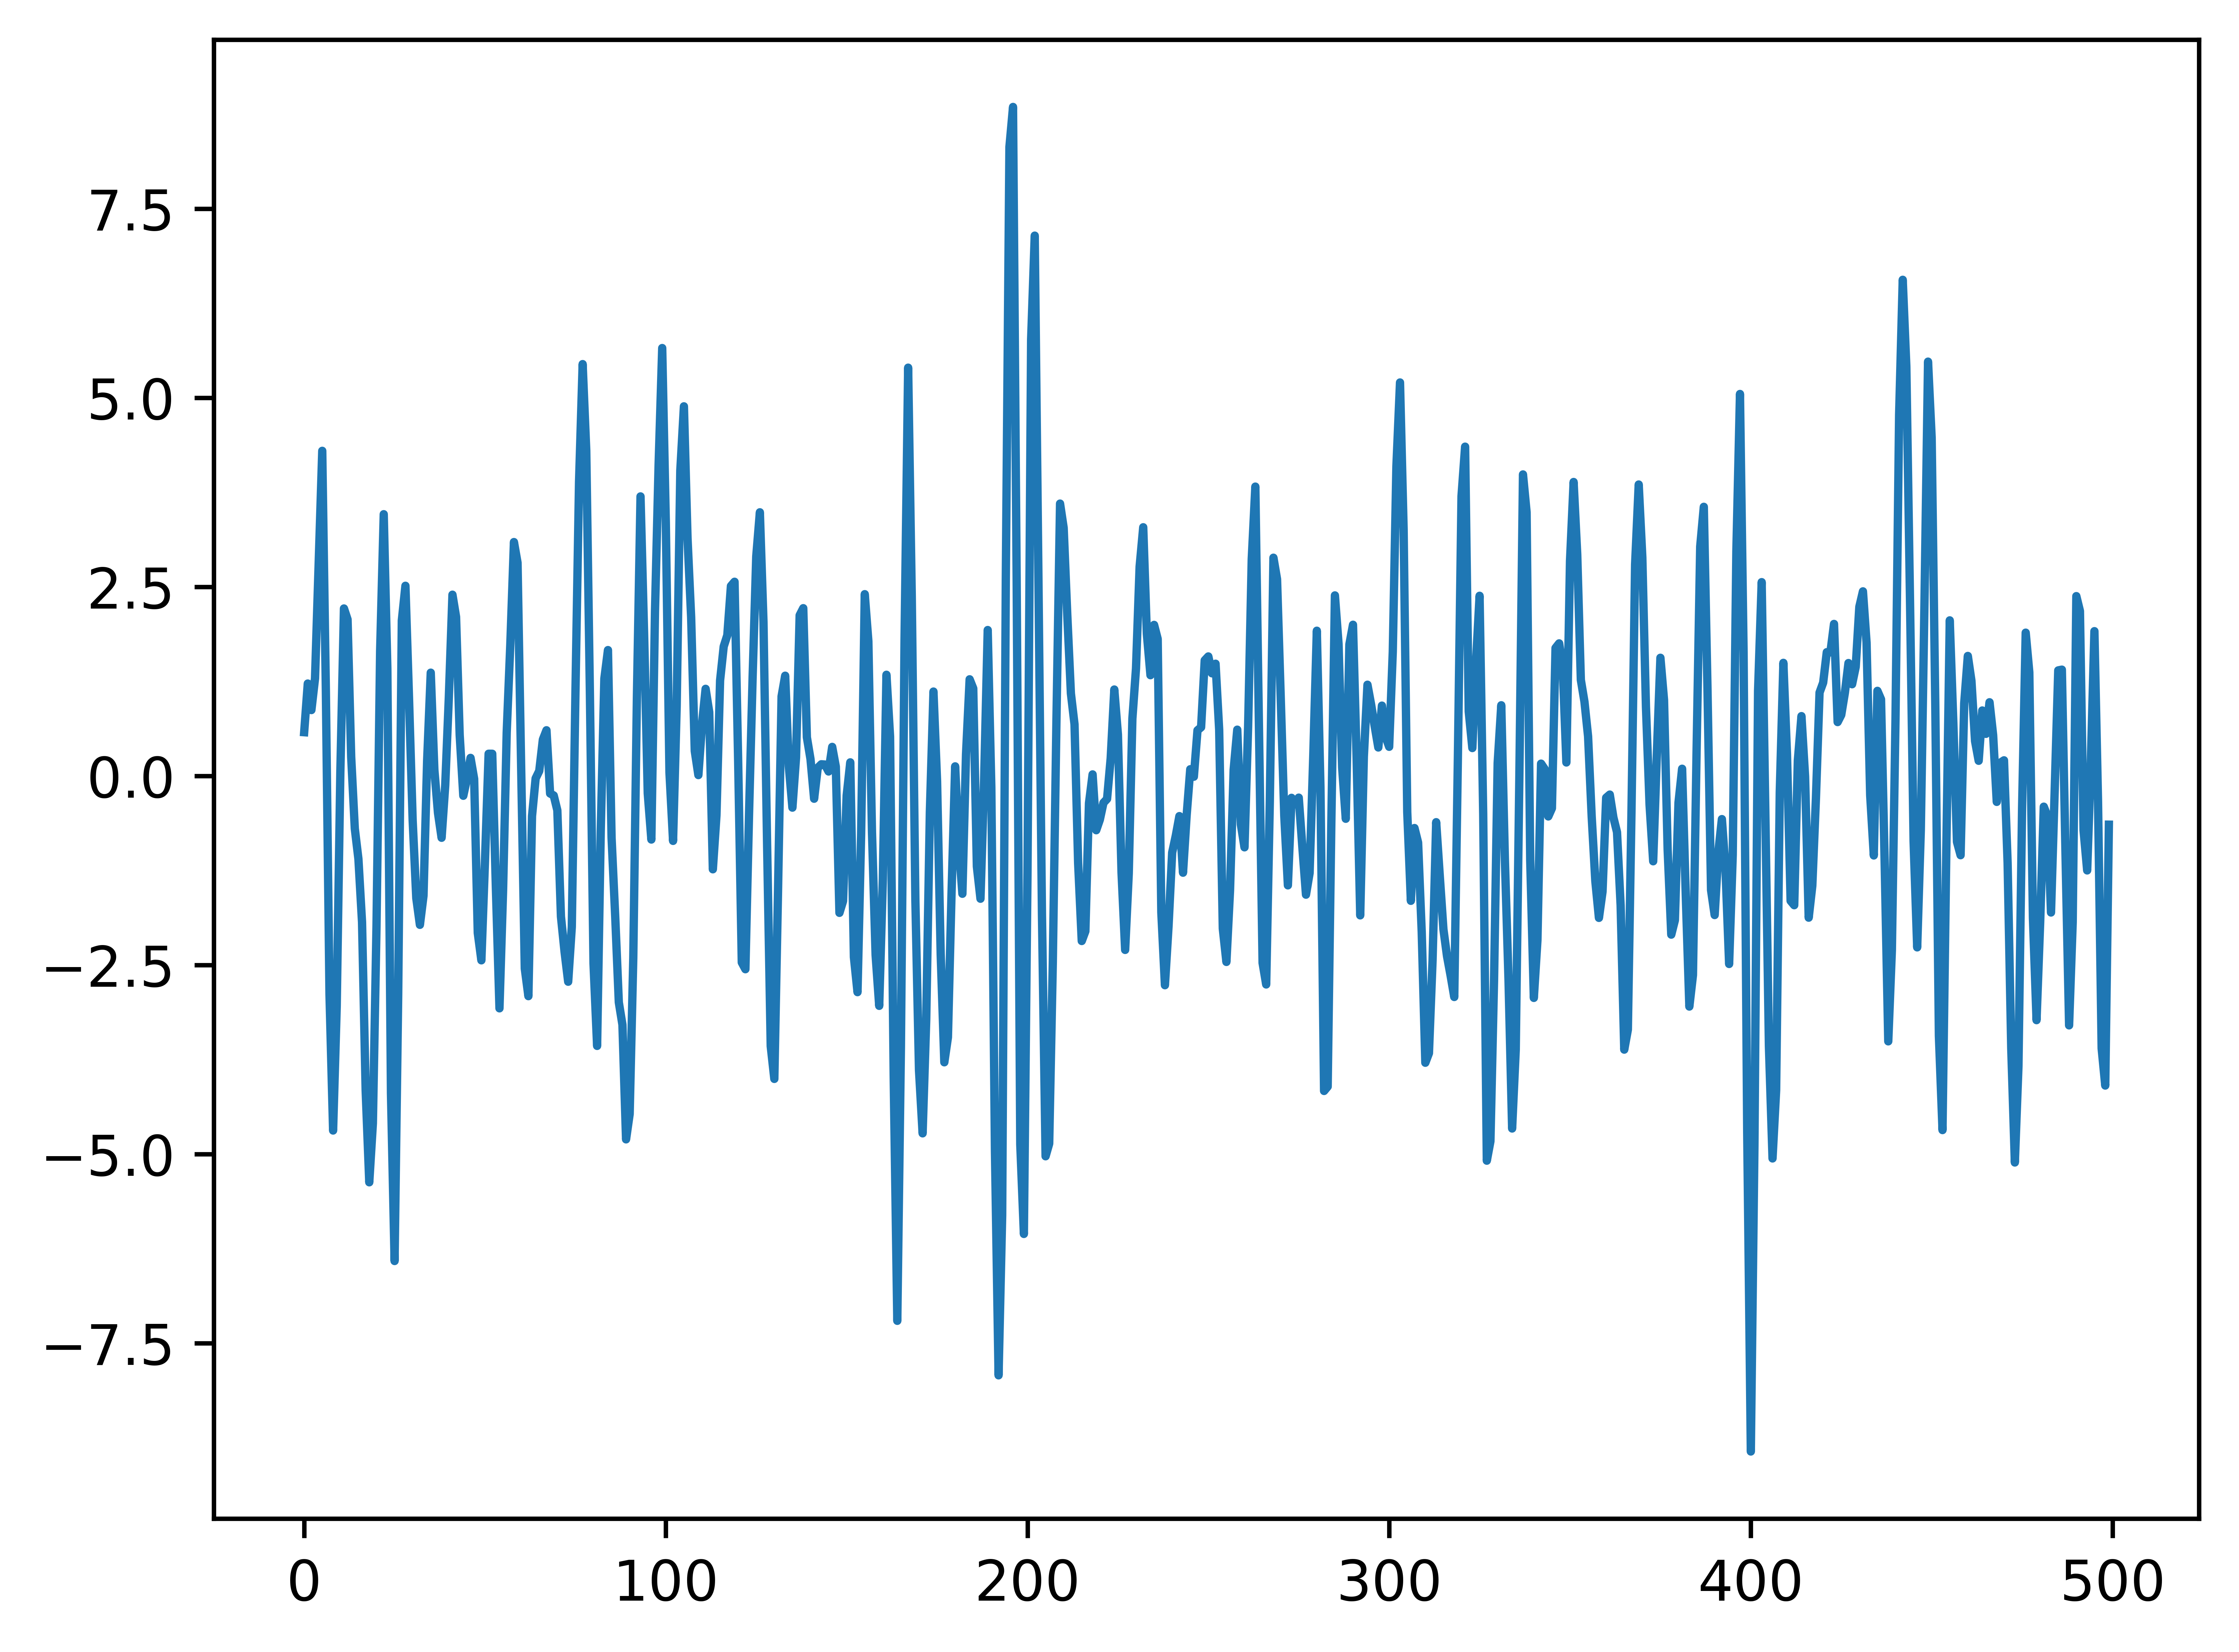
\includegraphics[height=7cm]{Graph1.png}
			\caption{Graph1}
			\label{fig: Graph1}
		\end{figure}
		\lipsum[1] 
		\vspace{0.7cm}\\
		\textcolor{red!75}{Equivalence between DC and SE}. Under usual
		regularity conditions (convexity and Inada conditions), and given
		$b^{i}(s^{0}) = \text{for all} \quad i \in I$, the allocations of the Debreu
		competitive equilibrium and the allocations of the sequential equilibrium
		are equivalent. Moreover, the spence of wages and interest rates are the same, and
			\begin{equation}\label{eq: DC and SE}
				Q(s^{t+1}|s^{t}) = \frac{q(s^{t+1})}{q(s^{t})} =
				\beta \frac{U_{c}^{i}(s^{t+1})}{U_{c}^{i}(s^{t})} \frac{\pi(s^{t+1})}{\pi(s^{t})}
			\end{equation}
		for all $ t, s^{t}$, and $s^{t+1}|s^{t}$.
		%% Tipo y nivel de investigación
		\subsection{Tipo y nivel de investigación}
			\lipsum[1]. Como se muestra el la ecuación \textcolor{blue}{\eqref{eq: MLG}}
			\begin{figure}[ht]
				\centering
				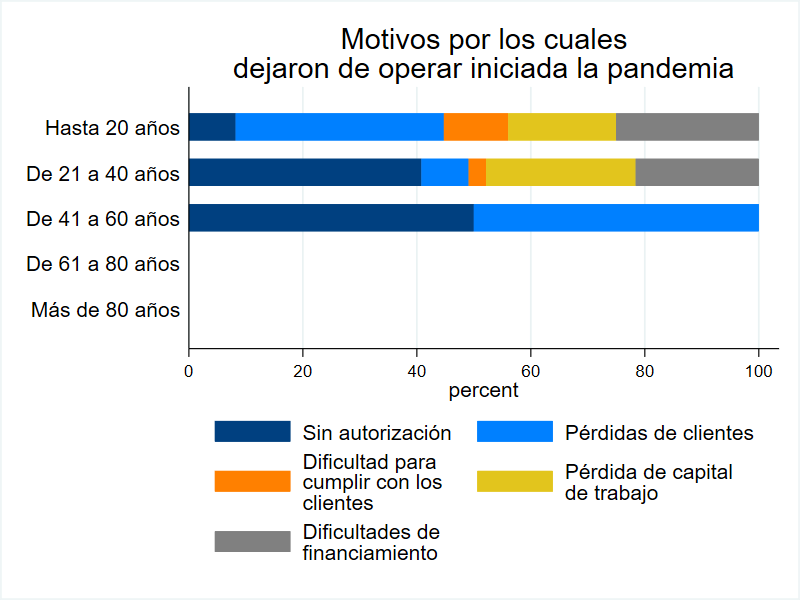
\includegraphics[height=7cm]{Graph2.png}
				\caption{Graph2}
				\label{fig: Graph2}
			\end{figure}
		%% Población y muestra
		\subsection{Población y muestra}
			\lipsum[1]. Como se muestra en la ecuación \textcolor{blue}{\eqref{eq: DC and SE}}. Asimismo, las figuras que se muestran a continuación fueron extraidos de \textcolor{blue}{\cite{Huang-2022}}.
			\begin{figure}[ht]
				\centering
				\begin{subfigure}[b]{0.3\textwidth}
					\centering
					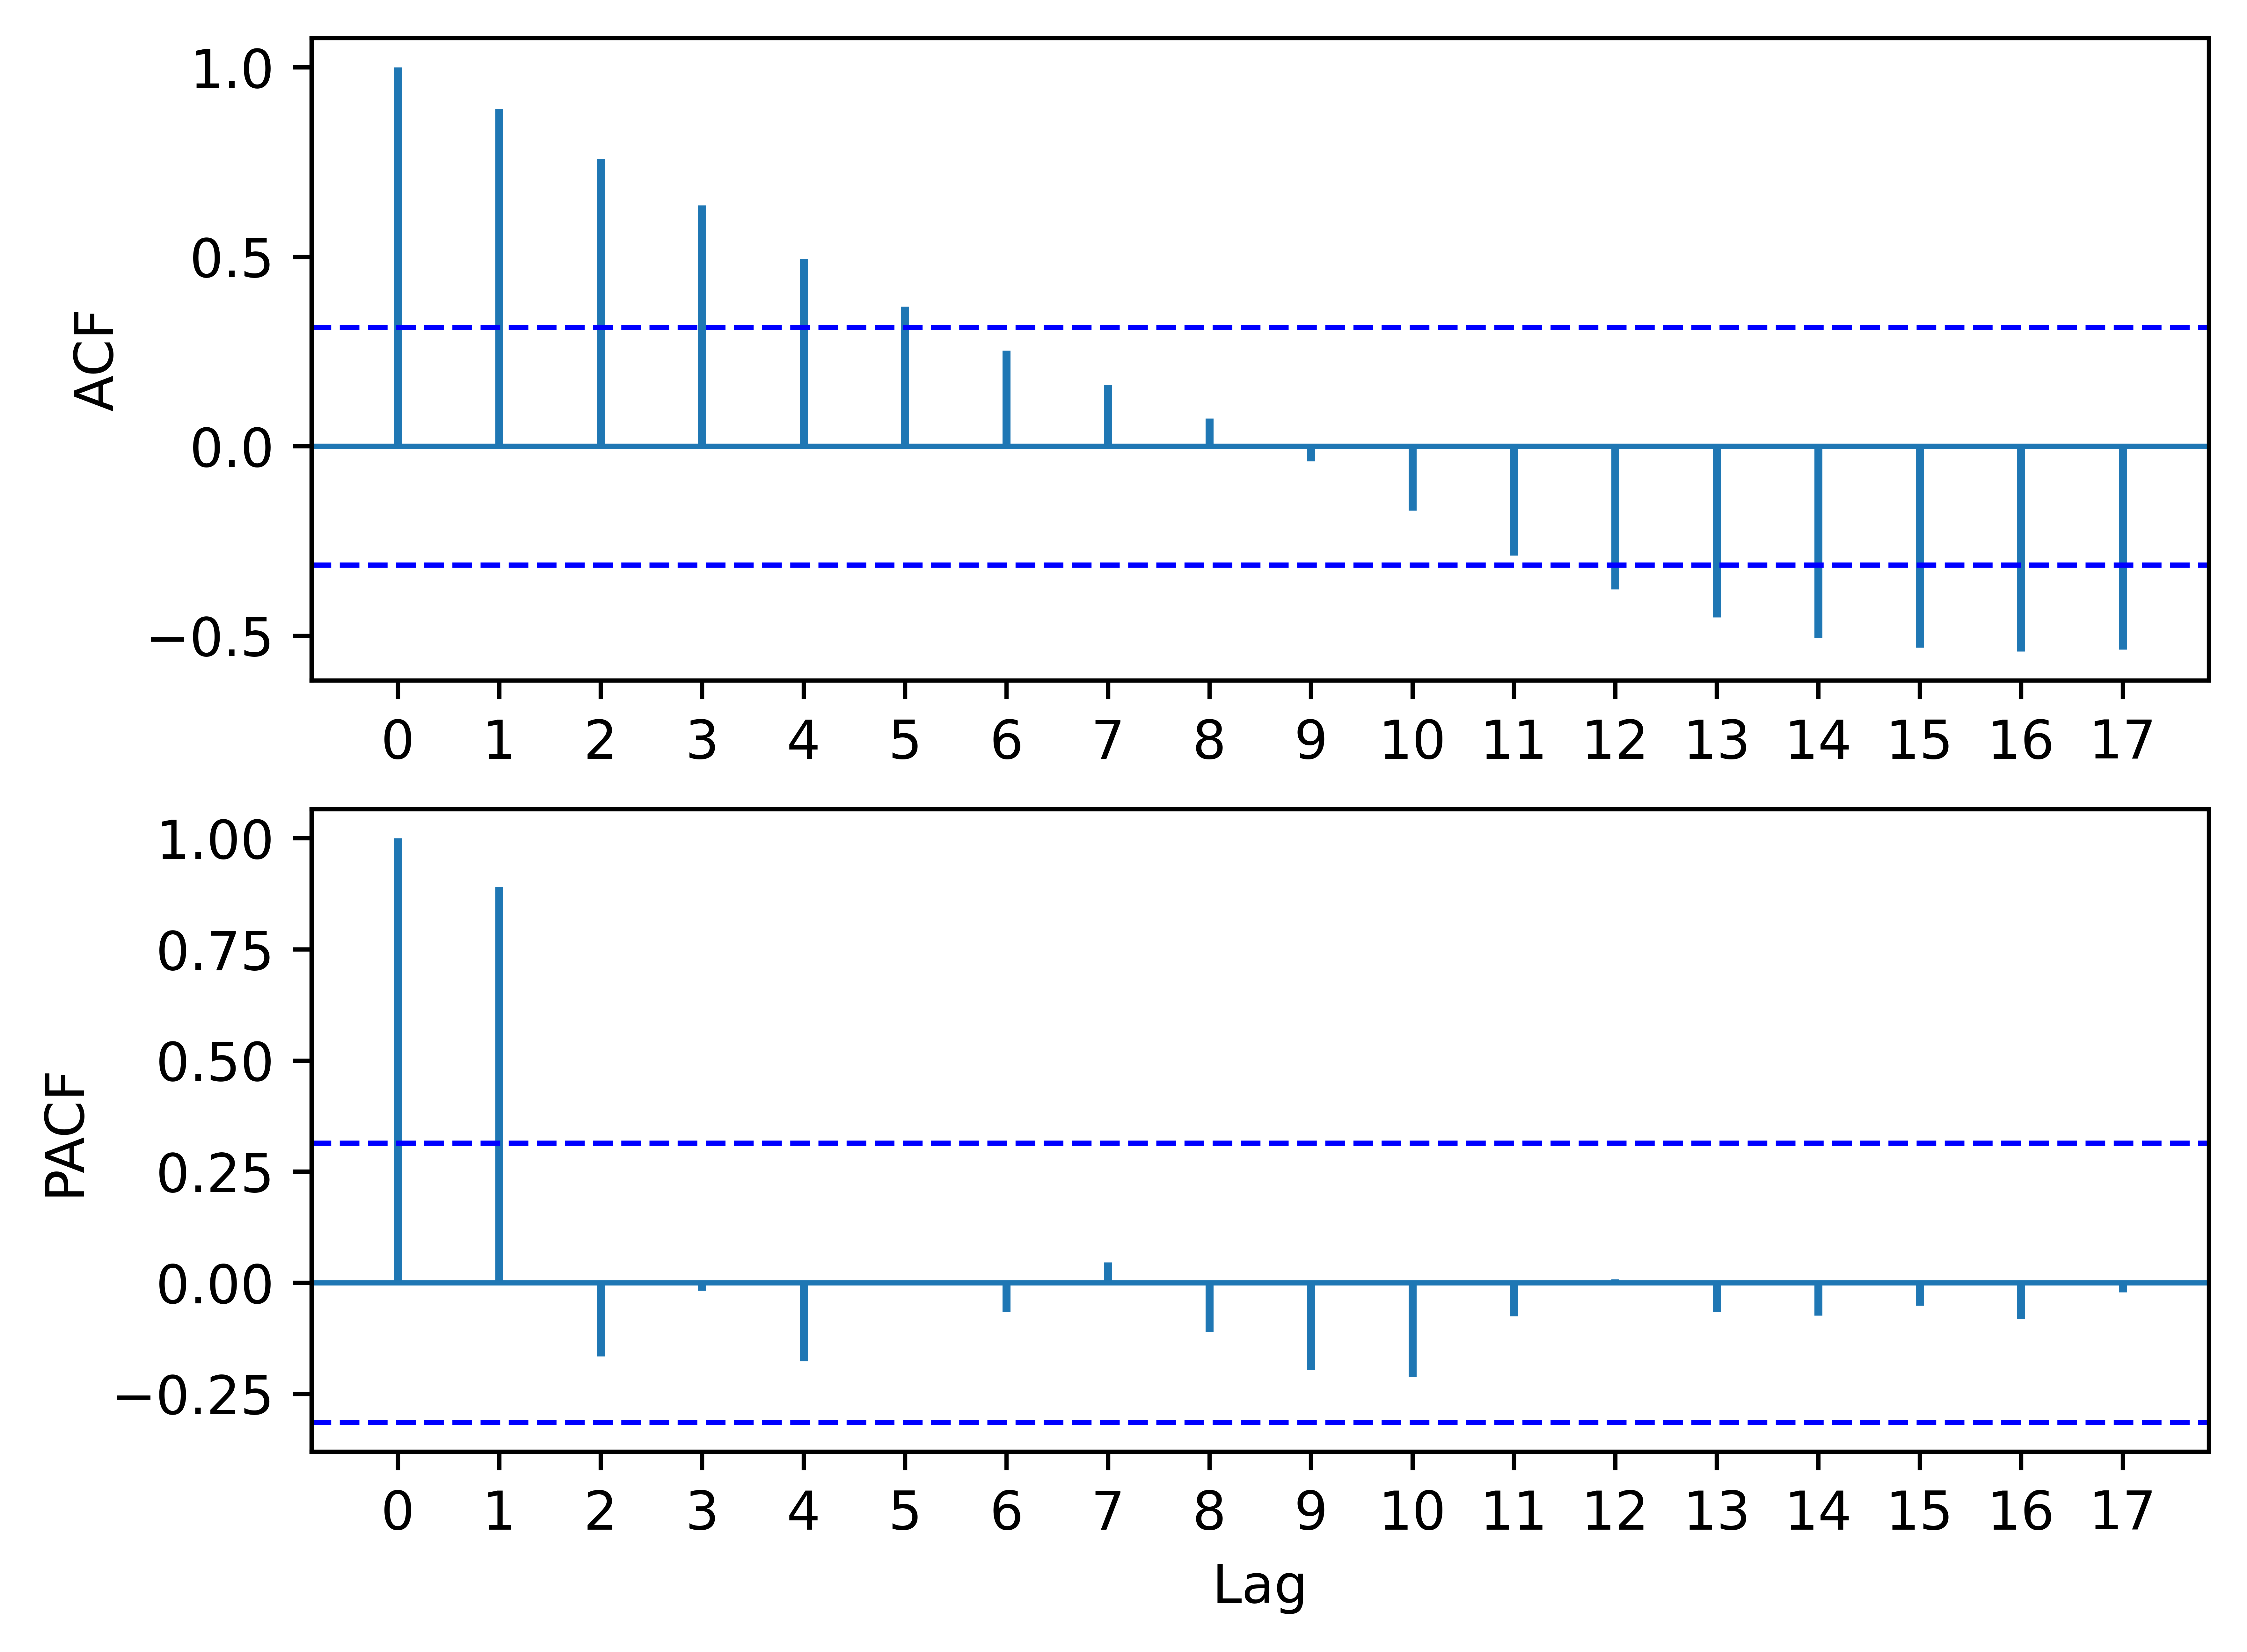
\includegraphics[width=\textwidth]{Graph6.png}
					\caption{Graph6}
					\label{subfig: Graph6}
				\end{subfigure}
				\hfill
				\begin{subfigure}[b]{0.3\textwidth}
					\centering
					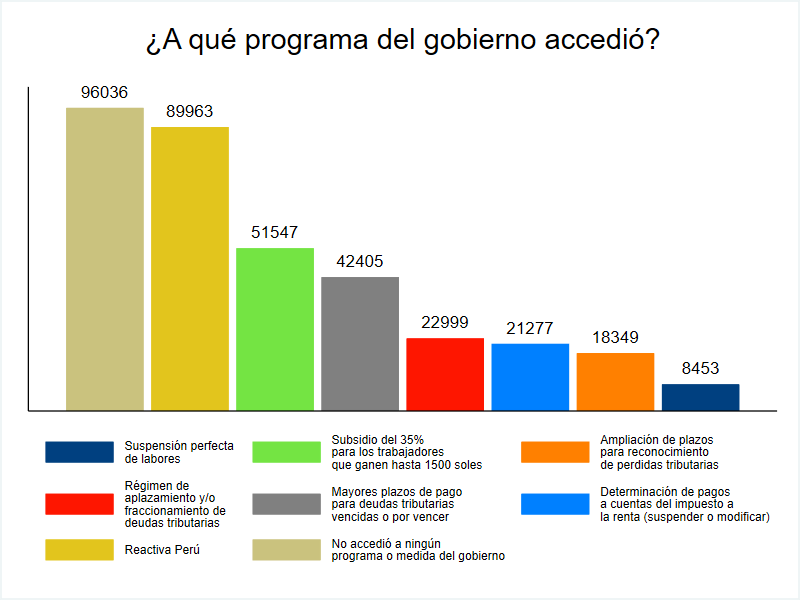
\includegraphics[width=\textwidth]{Graph4.png}
					\caption{Graph4}
					\label{subfig: Graph4}
				\end{subfigure}
				\hfill
				\begin{subfigure}[b]{0.3\textwidth}
					\centering
					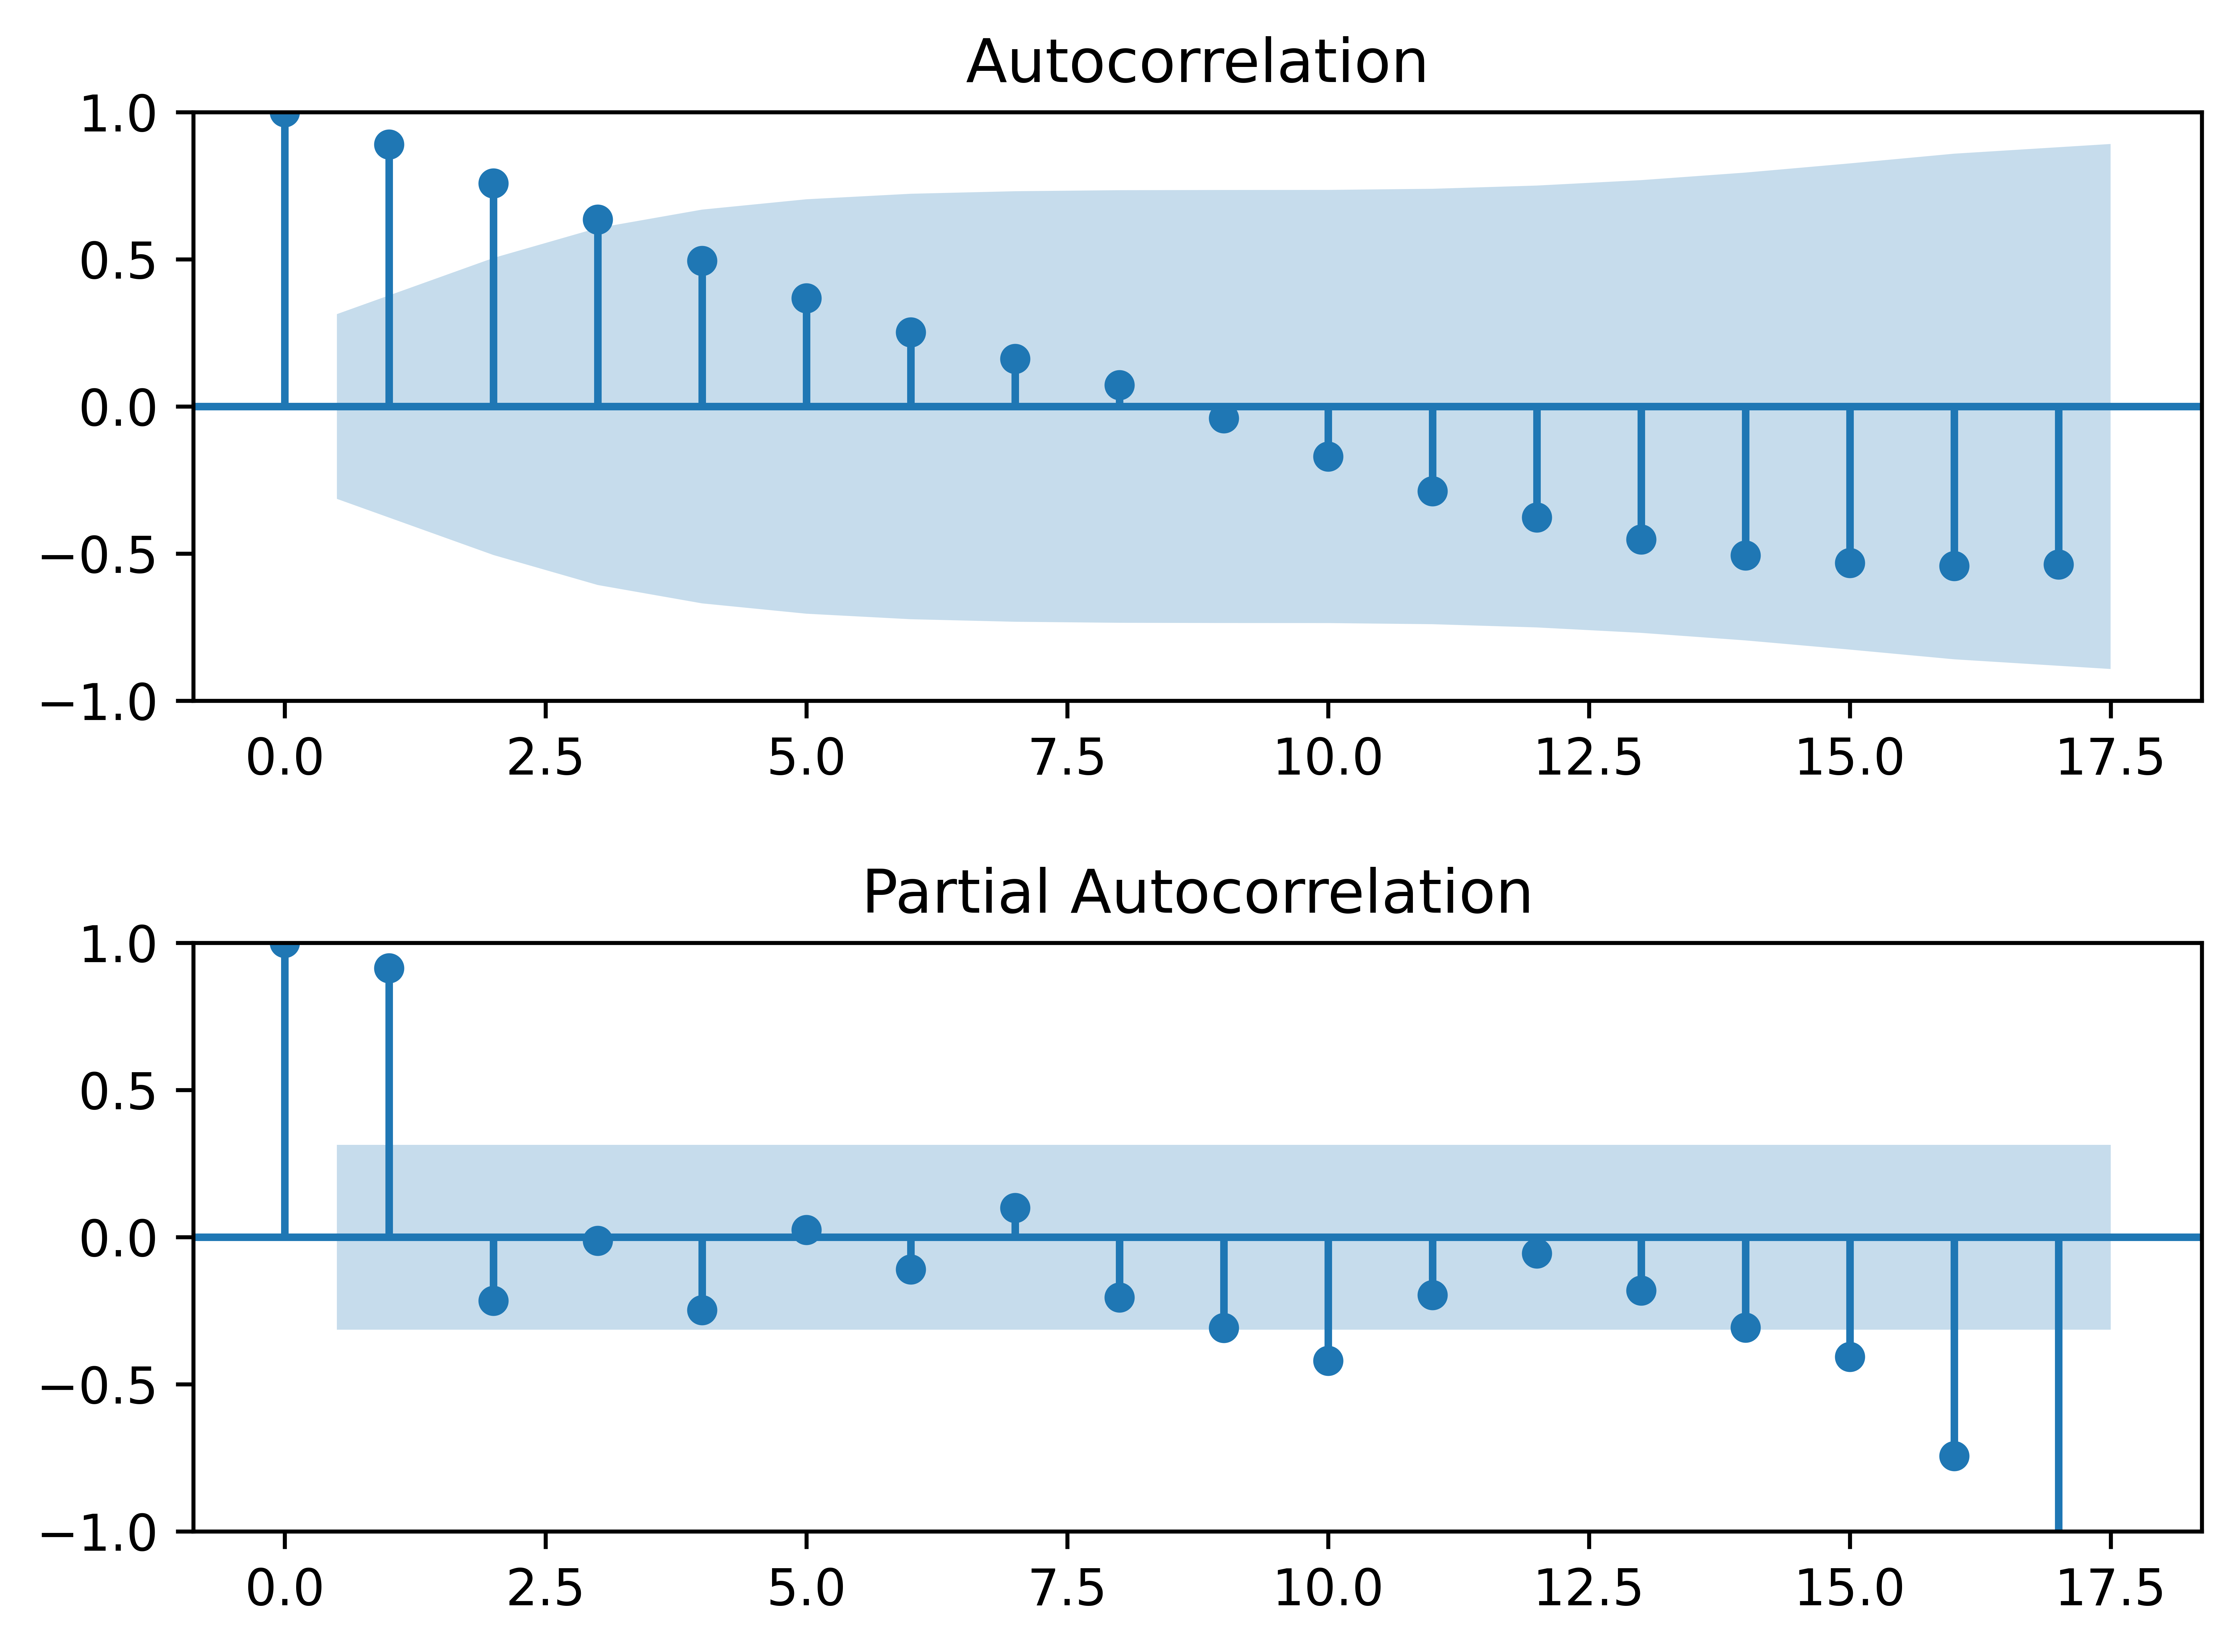
\includegraphics[width=\textwidth]{Graph5.png}
					\caption{Graph5}
					\label{subfig: Graph5}
				\end{subfigure}
				\caption{Graficas multiples}
				\label{fig: Graficas multiples}
			\end{figure}
		%% Fuentes de información
		\subsection{Fuentes de información}
			\lipsum[1]
			\begin{figure}[ht]
				\centering
				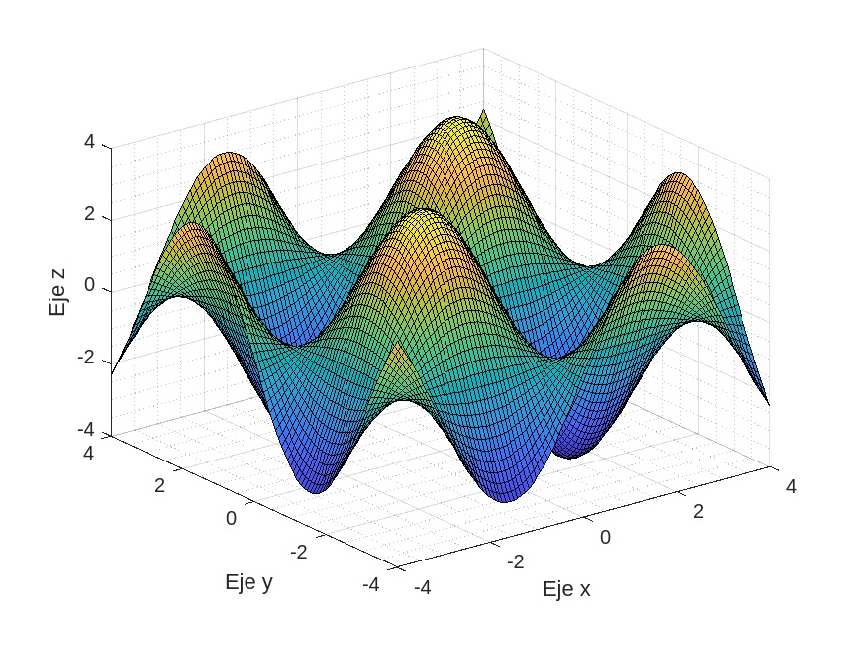
\includegraphics[height=7cm]{Graph3D.pdf}
				\caption{Graph3D}
				\label{fig: Graph3D}
			\end{figure}
		%% Diseño de investigación
		\subsection{Diseño de investigación}
			\lipsum[1]
			\begin{figure}[ht]
				\centering
				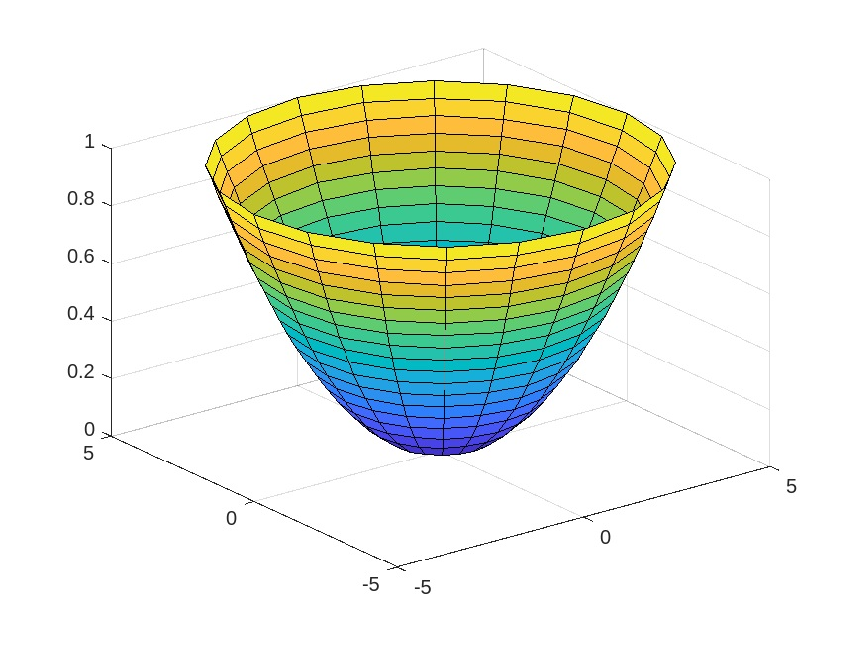
\includegraphics[height=7cm]{Graph3D_2.pdf}
				\caption{Graph3D-2}
				\label{fig: Graph3D-2}
			\end{figure}
		%% Técnicas e instrumentos
		\subsection{Técnicas e instrumentos}
			\lipsum[1]
			\begin{figure}[H]
				\centering
				\begin{tikzpicture}[scale = 1.8, samples = 70]
					\fill[green] (0,0) -- plot[domain = 0:pi] ({\x}, {sin(\x r)}) -- (pi,0) -- cycle;
					\fill[green] (pi,0) -- plot[domain = pi:2*pi] ({\x}, {sin(\x r)}) -- (2*pi,0) -- cycle;
					\draw[dashed, xstep = pi/2] (-pi/4, -1) grid (9*pi/4, 1);
					\draw[<-] (7,0) node[below right] {$x$} -- (-0.5,0); 
					\draw[<-] (0,1.25) node[above left] {$y$} -- (0, -1.25); 
					\node[below right] at (pi/2, 0) {$\frac{\pi}{2}$};
					\node[below right] at (pi, 0) {$\pi$};
					\node[below right] at (3*pi/2, 0) {$\frac{3\pi}{2}$};
					\node[below right] at (2*pi, 0) {$2\pi$};	
					\node[left] at (0,1) {$1$};
					\node[left] at (0,-1) {$-1$};
					\draw[very thick, azul, domain = -0.5 + 0:2*pi + 0.5] plot({\x}, {sin(\x r)}) node[right] {$h(x) = \sin x$};
					\draw[very thick, red, domain = -0.5 + 0:2*pi + 0.5] plot({\x}, {cos(\x r)}) node[above] {$g(x) = \cos x$};
				\end{tikzpicture}
				\caption{Función seno y coseno}
				\label{fig: Función seno}
			\end{figure}
		\lipsum[1].
	    \begin{equation}\label{eq: NL1}
	    	\alpha_{n}b_{n+1} + \beta_{n}b_{n} + \gamma_{n}b_{n-1} + \delta_{n}b_{n-2} +\varepsilon_{n}b_{n-3} = 0
	    \end{equation}
	    donde,
	    \begin{eqnarray}
	    	\alpha_{n} &=& \left(n+1\right)\left(n+1+|m|\right), \label{eq: NL2}\\
	    	\beta_{n} &=& -2n\left(2n+|m|\right) + m^{2}+|m| + k + \dfrac{a_{0}\in^{2}}{\ell^{2}}+\dfrac{2}{\ell}, \label{eq: NL3}\\
	    	\gamma_{n} &=& 6(n-1)^{2}-2\left(m^{2} + |m| + k + \dfrac{a_{0}^{2}\in^{2}}{\ell^{2}}\right), \label{eq: NL4} \\
	    	\delta_{n} &=& 2(n-2)\left(|m| - 2n + 4\right) + m^{2} + |m| + k + \dfrac{a_{0}\in^{2}}{\ell^{2}}-\dfrac{2}{\ell}, \label{eq: NL5}\\
	    	\varepsilon_{n} &=& (n-3)\left(n-3-|m|\right), \label{eq: NL6}
	    \end{eqnarray}
    	Estos resultados se pueden ver en \cite{Kim-2008}
	% Referencias bibliográficas
	\newpage
	\section{REFERENCIAS BIBLIOGRÁFICAS}
		%% Estilo APA
		\bibliography{Biblio.bib}
			%%% Style
			\bibliographystyle{apalike2}
	% Anexos
	\newpage
	\section{ANEXOS}
		%% Anexo 1
		\subsection{ANEXO 1: Matriz de consistencia}
			\begin{table}[H]
				\centering
				\caption{Matriz de consistencia}
				\begin{tabular}{p{5cm}p{5cm}p{5cm}}
					\hline
					Problema & Objetivo & Hipótesis\\
					\hline
					\lipsum[1] & \lipsum[1] & \lipsum[1]\\
					\hline
				\end{tabular}
				\vspace{2mm}
				\caption*{\it Nota: Elaboración propia.}
				\label{tab: Matriz de consistencia}
			\end{table}
		%% Anexo 2
		\newpage
		\subsection{ANEXO 2: Resultados }
			\begin{table}[H]
				\centering
				\caption{Tabla de resultados}
				\begin{tabular}{p{5cm}p{5cm}p{5cm}}
					\hline
					Resultado 1 & Resultado 2 & Resultado 3\\
					\hline
					\lipsum[1] & \lipsum[1] & \lipsum[1]\\
					\hline
				\end{tabular}
				\vspace{2mm}
				\caption*{\it Nota: Elaboración propia.}
				\label{tab: Resultados}
			\end{table}
		%% Anexo 3
		\newpage
		\subsection{ANEXO 3: Datos }
			\begin{table}[H]
				\centering
				\caption{Datos}
				\begin{tabular}{p{5cm}p{5cm}p{5cm}}
					\hline
					Variable 1 & Variable 2 & Varaible 3\\
					\hline
					\lipsum[1] & \lipsum[1] & \lipsum[1]\\
					\hline
				\end{tabular}
				\vspace{2mm}
				\caption*{\it Nota: Elaboración propia.}
				\label{tab: Datos}
			\end{table}
		%% Anexo 4
		\newpage 
		\subsection{ANEXO 4: Código de Matlab}
	    	\lstinputlisting[language=Matlab]{ProgramsCode/MatlabCode.m}
	    %% Anexo 5
	    \newpage
	    \subsection{ANEXO 5: Código de Java}
	    	\lstinputlisting[language=Java]{ProgramsCode/JavaCode.java}
	    %% Anexo 6
	    \newpage
	    \subsection{ANEXO 6: Código de Python}
		 	\lstinputlisting[language=Python]{ProgramsCode/PythonCode.py}
\end{document}
